%\documentclass{beamer} 
\documentclass[handout]{beamer} % sin pausas
\usetheme{CambridgeUS}
%\setbeamertemplate{background}[grid][step=8 ] % cuadriculado

\usepackage{etex}
\usepackage{t1enc}
\usepackage[spanish,es-nodecimaldot]{babel}
\usepackage{latexsym}
\usepackage[utf8]{inputenc}
\usepackage{verbatim}
\usepackage{multicol}
\usepackage{amsgen,amsmath,amstext,amsbsy,amsopn,amsfonts,amssymb}
\usepackage{amsthm}
\usepackage{calc}         % From LaTeX distribution
\usepackage{graphicx}     % From LaTeX distribution
\usepackage{ifthen}
%\usepackage{makeidx}
\input{random.tex}        % From CTAN/macros/generic
\usepackage{subfigure} 
\usepackage{tikz}
\usepackage[customcolors]{hf-tikz}
\usetikzlibrary{arrows}
\usetikzlibrary{matrix}
\tikzset{
	every picture/.append style={
		execute at begin picture={\deactivatequoting},
		execute at end picture={\activatequoting}
	}
}
\usetikzlibrary{decorations.pathreplacing,angles,quotes}
\usetikzlibrary{shapes.geometric}
\usepackage{mathtools}
\usepackage{stackrel}
%\usepackage{enumerate}
\usepackage{enumitem}
\usepackage{tkz-graph}
\usepackage{polynom}
\polyset{%
	style=B,
	delims={(}{)},
	div=:
}
\renewcommand\labelitemi{$\circ$}
\setlist[enumerate]{label={(\arabic*)}}
\setbeamertemplate{itemize item}{$\circ$}
\setbeamertemplate{enumerate items}[default]
\definecolor{links}{HTML}{2A1B81}
\hypersetup{colorlinks,linkcolor=,urlcolor=links}


\newcommand{\Id}{\operatorname{Id}}
\newcommand{\img}{\operatorname{Im}}
\newcommand{\nuc}{\operatorname{Nu}}
\newcommand{\im}{\operatorname{Im}}
\renewcommand\nu{\operatorname{Nu}}
\newcommand{\la}{\langle}
\newcommand{\ra}{\rangle}
\renewcommand{\t}{{\operatorname{t}}}
\renewcommand{\sin}{{\,\operatorname{sen}}}
\newcommand{\Q}{\mathbb Q}
\newcommand{\R}{\mathbb R}
\newcommand{\C}{\mathbb C}
\newcommand{\K}{\mathbb K}
\newcommand{\F}{\mathbb F}
\newcommand{\Z}{\mathbb Z}
\newcommand{\N}{\mathbb N}
\newcommand\sgn{\operatorname{sgn}}
\renewcommand{\t}{{\operatorname{t}}}
\renewcommand{\figurename }{Figura}

%
% Ver http://joshua.smcvt.edu/latex2e/_005cnewenvironment-_0026-_005crenewenvironment.html
%

\renewenvironment{block}[1]% environment name
{% begin code
	\par\vskip .2cm%
	{\color{blue}#1}%
	\vskip .2cm
}%
{%
	\vskip .2cm}% end code


\renewenvironment{alertblock}[1]% environment name
{% begin code
	\par\vskip .2cm%
	{\color{red!80!black}#1}%
	\vskip .2cm
}%
{%
	\vskip .2cm}% end code


\renewenvironment{exampleblock}[1]% environment name
{% begin code
	\par\vskip .2cm%
	{\color{blue}#1}%
	\vskip .2cm
}%
{%
	\vskip .2cm}% end code




\newenvironment{exercise}[1]% environment name
{% begin code
	\par\vspace{\baselineskip}\noindent
	\textbf{Ejercicio (#1)}\begin{itshape}%
		\par\vspace{\baselineskip}\noindent\ignorespaces
	}%
	{% end code
	\end{itshape}\ignorespacesafterend
}


\newenvironment{definicion}[1][]% environment name
{% begin code
	\par\vskip .2cm%
	{\color{blue}Definición #1}%
	\vskip .2cm
}%
{%
	\vskip .2cm}% end code

    \newenvironment{notacion}[1][]% environment name
    {% begin code
        \par\vskip .2cm%
        {\color{blue}Notación #1}%
        \vskip .2cm
    }%
    {%
        \vskip .2cm}% end code

\newenvironment{observacion}[1][]% environment name
{% begin code
	\par\vskip .2cm%
	{\color{blue}Observación #1}%
	\vskip .2cm
}%
{%
	\vskip .2cm}% end code

\newenvironment{ejemplo}[1][]% environment name
{% begin code
	\par\vskip .2cm%
	{\color{blue}Ejemplo #1}%
	\vskip .2cm
}%
{%
	\vskip .2cm}% end code


\newenvironment{preguntas}[1][]% environment name
{% begin code
    \par\vskip .2cm%
    {\color{blue}Preguntas #1}%
    \vskip .2cm
}%
{%
    \vskip .2cm}% end code

\newenvironment{ejercicio}[1][]% environment name
{% begin code
	\par\vskip .2cm%
	{\color{blue}Ejercicio #1}%
	\vskip .2cm
}%
{%
	\vskip .2cm}% end code


\renewenvironment{proof}% environment name
{% begin code
	\par\vskip .2cm%
	{\color{blue}Demostración}%
	\vskip .2cm
}%
{%
	\vskip .2cm}% end code



\newenvironment{demostracion}% environment name
{% begin code
	\par\vskip .2cm%
	{\color{blue}Demostración}%
	\vskip .2cm
}%
{%
	\vskip .2cm}% end code

\newenvironment{idea}% environment name
{% begin code
	\par\vskip .2cm%
	{\color{blue}Idea de la demostración}%
	\vskip .2cm
}%
{%
	\vskip .2cm}% end code

\newenvironment{solucion}% environment name
{% begin code
	\par\vskip .2cm%
	{\color{blue}Solución}%
	\vskip .2cm
}%
{%
	\vskip .2cm}% end code



\newenvironment{lema}[1][]% environment name
{% begin code
	\par\vskip .2cm%
	{\color{blue}Lema #1}\begin{itshape}%
		\par\vskip .2cm
	}%
	{% end code
	\end{itshape}\vskip .2cm\ignorespacesafterend
}

\newenvironment{proposicion}[1][]% environment name
{% begin code
	\par\vskip .2cm%
	{\color{blue}Proposición #1}\begin{itshape}%
		\par\vskip .2cm
	}%
	{% end code
	\end{itshape}\vskip .2cm\ignorespacesafterend
}

\newenvironment{teorema}[1][]% environment name
{% begin code
	\par\vskip .2cm%
	{\color{blue}Teorema #1}\begin{itshape}%
		\par\vskip .2cm
	}%
	{% end code
	\end{itshape}\vskip .2cm\ignorespacesafterend
}


\newenvironment{corolario}[1][]% environment name
{% begin code
	\par\vskip .2cm%
	{\color{blue}Corolario #1}\begin{itshape}%
		\par\vskip .2cm
	}%
	{% end code
	\end{itshape}\vskip .2cm\ignorespacesafterend
}

\newenvironment{propiedad}% environment name
{% begin code
	\par\vskip .2cm%
	{\color{blue}Propiedad}\begin{itshape}%
		\par\vskip .2cm
	}%
	{% end code
	\end{itshape}\vskip .2cm\ignorespacesafterend
}

\newenvironment{conclusion}% environment name
{% begin code
	\par\vskip .2cm%
	{\color{blue}Conclusión}\begin{itshape}%
		\par\vskip .2cm
	}%
	{% end code
	\end{itshape}\vskip .2cm\ignorespacesafterend
}


\newenvironment{definicion*}% environment name
{% begin code
	\par\vskip .2cm%
	{\color{blue}Definición}%
	\vskip .2cm
}%
{%
	\vskip .2cm}% end code

\newenvironment{observacion*}% environment name
{% begin code
	\par\vskip .2cm%
	{\color{blue}Observación}%
	\vskip .2cm
}%
{%
	\vskip .2cm}% end code


\newenvironment{obs*}% environment name
	{% begin code
		\par\vskip .2cm%
		{\color{blue}Observación}%
		\vskip .2cm
	}%
	{%
		\vskip .2cm}% end code

\newenvironment{ejemplo*}% environment name
{% begin code
	\par\vskip .2cm%
	{\color{blue}Ejemplo}%
	\vskip .2cm
}%
{%
	\vskip .2cm}% end code

\newenvironment{ejercicio*}% environment name
{% begin code
	\par\vskip .2cm%
	{\color{blue}Ejercicio}%
	\vskip .2cm
}%
{%
	\vskip .2cm}% end code

\newenvironment{propiedad*}% environment name
{% begin code
	\par\vskip .2cm%
	{\color{blue}Propiedad}\begin{itshape}%
		\par\vskip .2cm
	}%
	{% end code
	\end{itshape}\vskip .2cm\ignorespacesafterend
}

\newenvironment{conclusion*}% environment name
{% begin code
	\par\vskip .2cm%
	{\color{blue}Conclusión}\begin{itshape}%
		\par\vskip .2cm
	}%
	{% end code
	\end{itshape}\vskip .2cm\ignorespacesafterend
}






\newcommand{\nc}{\newcommand}

%%%%%%%%%%%%%%%%%%%%%%%%%LETRAS

\nc{\FF}{{\mathbb F}} \nc{\NN}{{\mathbb N}} \nc{\QQ}{{\mathbb Q}}
\nc{\PP}{{\mathbb P}} \nc{\DD}{{\mathbb D}} \nc{\Sn}{{\mathbb S}}
\nc{\uno}{\mathbb{1}} \nc{\BB}{{\mathbb B}} \nc{\An}{{\mathbb A}}

\nc{\ba}{\mathbf{a}} \nc{\bb}{\mathbf{b}} \nc{\bt}{\mathbf{t}}
\nc{\bB}{\mathbf{B}}

\nc{\cP}{\mathcal{P}} \nc{\cU}{\mathcal{U}} \nc{\cX}{\mathcal{X}}
\nc{\cE}{\mathcal{E}} \nc{\cS}{\mathcal{S}} \nc{\cA}{\mathcal{A}}
\nc{\cC}{\mathcal{C}} \nc{\cO}{\mathcal{O}} \nc{\cQ}{\mathcal{Q}}
\nc{\cB}{\mathcal{B}} \nc{\cJ}{\mathcal{J}} \nc{\cI}{\mathcal{I}}
\nc{\cM}{\mathcal{M}} \nc{\cK}{\mathcal{K}}

\nc{\fD}{\mathfrak{D}} \nc{\fI}{\mathfrak{I}} \nc{\fJ}{\mathfrak{J}}
\nc{\fS}{\mathfrak{S}} \nc{\gA}{\mathfrak{A}}
%%%%%%%%%%%%%%%%%%%%%%%%%LETRAS



\title[Clase 6 - Conteo]{Matemática Discreta I \\ Clase 6 - Conteo}
%\author[C. Olmos / A. Tiraboschi]{Carlos Olmos / Alejandro Tiraboschi}
\institute[]{\normalsize FAMAF / UNC
	\\[\baselineskip] ${}^{}$
	\\[\baselineskip]
}
\date[06/04/2021]{6 de abril  de 2021}




\begin{document}
%\title{El centro geográfico de Argentina}   
%\author{} 
%\date{Villa Huidobro \\ 4/12/2018} 



\frame{\titlepage} 

%\frame{\frametitle{Índice}\tableofcontents} 




\begin{frame}\frametitle{Cardinal de un conjunto } 	

	Un conjunto $A$ es finito si podemos contar la cantidad de elementos que tiene. En ese caso denotaremos $|A|$ la cantidad de elementos de $A$ y la llamaremos el {\em cardinal de $A$}\
	\pause
   \vskip .6cm
   Por  ejemplo, los conjuntos
   \begin{equation*}
   	A = \{ a, b, z, x, 1\}, \qquad B = \{ 1, 2, 3, 4, 5\}
   \end{equation*}
   tienen 5 elementos cada uno. Es decir $|A| =5$ y $|B|= 5$.
   
   \vskip .6cm\pause
   
   Conjuntos como $\mathbb Z$, $\mathbb N$ o $\mathbb R$ son infinitos y por lo tanto no tiene sentido hablar de la cantidad de elementos de estos conjuntos.
\end{frame}

\begin{frame}\frametitle{El principio de adición} 	   
	Dadas dos actividades $X$ e $Y$, si se puede realizar $X$ de $n$ formas distintas o, alternativamente, se puede realizar  $Y$ de $m$ formas distintas. Entonces el número de formas de realizar ``$X$ o $Y$'' es $n + m$.

	\pause
	 \vskip .4cm
	 {\color{blue} Ejemplo}
	 \vskip .2cm 
	 Supongamos que una persona va a salir a pasear  y puede ir al cine donde hay $3$ películas en cartel o al teatro donde hay $4$ obras posibles. Entonces, tendrá un total de $3+4=7$ formas distintas de elegir el paseo. 
	  \vskip .3cm
	 

	
	

\end{frame}


\begin{frame}
	Este principio, el {\it principio de adición}, es el más básico del conteo y más formalmente dice que si $A$ y $B$ son conjuntos finitos disjuntos, entonces 
\begin{equation*}\label{padd}
|A \cup B| =|A|+|B|.
\end{equation*}
  \vskip .4cm  \pause
 Se generaliza fácilmente:  
Sean $A_1,\ldots,A_n$ conjuntos finitos tal que $A_i \cap A_j = \emptyset$ cuando $i\not=j$, entonces 
\begin{equation*}
|A_1 \cup \cdots \cup A_n| =|A_1|+\cdots+|A_n|.
\end{equation*}
\pause

\vskip .4cm

Remarcamos que para aplicar el principio de adición es necesario que los eventos se { \bf excluyan mutuamente}. El caso general es
\begin{equation*}
	|A \cup B| =|A|+|B| - |A \cap B|.
\end{equation*}

\end{frame}

\begin{frame}\frametitle{El principio de multiplicación} 
		Suponga que una actividad consiste de $2$ etapas y la primera etapa puede ser realizada de $n_1$ maneras y la etapa $2$  puede realizarse de $n_2$  maneras, independientemente de como se ha hecho la etapa $1$. 
		\vskip .2cm
		{\it Principio de multiplicación:} la actividad puede ser realizada de $n_1\cdot n_2$  formas distintas.
		
	\pause 	
	\vskip .6cm
	{\color{blue} Ejemplo}
	\vskip .2cm
			Supongamos que la persona del ejemplo anterior tiene suficiente tiempo y dinero para ir primero al cine (3 posibilidades) y luego al teatro (4 posibilidades). 
			\vskip .2cm
			Entonces tendrá  $3 \cdot 4=12$ formas distintas de hacer el paseo.

	 
	
		
		
\end{frame}

\begin{frame}
		
	Formalmente, si $A,B$ conjuntos y definimos el {\em producto cartesiano}\index{producto cartesiano} entre $A$ y $B$ por
	$$
	A \times B = \{(a,b): a \in A, b \in B\}.
	$$
		\vskip .5cm
		
		
	Entonces si $A$ y $B$ son conjuntos finitos se cumple que
	$$
	|A \times B| = |A|\cdot|B|.  
	$$
	
			\vskip .3cm 		
	{\bf Caso  especial:} $A = B$.
	\pause 
	\vskip .3cm
	{\color{blue} Ejemplo}
	\vskip .2cm
	
	¿Cuántas palabras de dos letras hay? (26 letras,  no importa si tienen significado)
	\pause
	
	\vskip .2cm
	
	
	{\color{blue} Respuesta:} $26 \cdot 26$.
	\vskip .2cm
	
\end{frame}

\begin{frame}\frametitle{Selecciones ordenadas con repetición}


{\color{blue} Ejemplo}
\vskip .2cm

 Sea  $X = \{ 1, 2, 3 \}$.
 \vskip .2cm
 ¿De cuántas formas se pueden elegir dos de estos números en forma ordenada?
	\vskip .2cm
{\bf Notación:} si elegimos $a$ y $b$ en forma ordenada, denotamos $ab$. 
     \vskip .2cm
Entonces, las posibilidades son 
	\begin{align*}
	&11&\quad &12&\quad &13 \\
	&21&\quad &22&\quad &23\\
	&31&\quad &32&\quad &33
	\end{align*}
	
	 \vskip .1cm 
	Es decir, hay $9 = 3^2$ formas posibles. 
	
	 \vskip .2cm ¿Cómo justificamos esto? \pause Por el principio de multiplicación


\end{frame}

\begin{frame}	

	
Avancemos un poco más y ahora elijamos en forma ordenada $3$ elementos de  ${1,2,3}$, es claro que estas elecciones son
\begin{align*}
&1 1 1&\quad &211&\quad &311 \\
&1 1 2&\quad & 212&\quad & 312\\
&1 1 3&\quad & 213&\quad & 313\\
&1 2 1&\quad & 221&\quad & 321\\
&1 2 2&\quad & 222&\quad & 322\\
&1 2 3&\quad & 223&\quad & 323\\
&1 3 1&\quad & 231&\quad & 331\\
&1 3 2&\quad & 232&\quad & 332\\
&1 3 3&\quad & 233&\quad & 333.
\end{align*}
El total de elecciones posibles $27 = 3^3$. 




\end{frame}

\begin{frame}	
	

Un diagrama arbolado ayuda a pensar. \pause
\begin{center}
	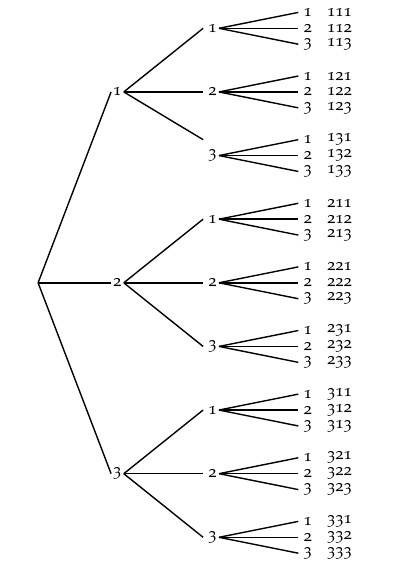
\includegraphics[scale=0.50]{images/arbol_pos.jpg}
\end{center}

%\vskip 8cm
\end{frame}



\begin{frame}	

	
El razonamiento anterior  se puede extender:

%\begin{proposicion}
\vskip .3cm
{\color{blue} Proposición}
\vskip .2cm
	{\it  Sean  $m,n \in \mathbb N$. Hay   $n^m$ formas posibles de elegir ordenadamente $m$ elementos de un conjunto de $n$ elementos.}
%\end{proposicion}
\vskip .5cm \pause
{\color{blue} Idea de la prueba.} \pause
\vskip .2cm
%\begin{proof}[Idea de la prueba]
	La prueba de esta proposición se basa en aplicar el principio de multiplicación $m-1$ veces, 
	\vskip .2cm
	A nivel formal,  debemos hacer inducción sobre $m$ y usar el principio de multiplicación en el paso inductivo. 

    \qed
%\end{proof}

\end{frame}



\begin{frame}	


%\begin{ejemplo}
	\vskip .3cm
	{\color{blue} Ejemplo}
	\vskip .2cm
	¿Cuántos números de cuatro dígitos pueden formarse con
	los dígitos $1, 2, 3, 4, 5, 6$?
	\vskip .2cm \pause
	Por la proposición anterior es claro que hay $6^4$ números posibles.
%\end{ejemplo}

%\begin{ejemplo}
\pause
\vskip .8cm
{\color{blue} Ejemplo}
\vskip .2cm
	¿Cuántos números de $5$ dígitos y capicúas pueden formarse
	con los dígitos $1, 2, 3, 4, 5, 6, 7, 8$? 
	\vskip .2cm \pause
	Un número
	capicúa de cinco dígitos es de la forma
	$$xyzyx$$
	Se reduce a ver cuántos números de tres dígitos pueden
	formarse con aquéllos dígitos. \pause
	Exactamente $8^3$.
%\end{ejemplo}

\end{frame}

\begin{frame}
	
	
		{\color{blue} Ejemplo}
		\vskip .2cm
Sea $X$ un conjunto de $n$ elementos. ¿Cuántos subconjuntos tiene este conjunto?
\vskip .2cm
Por ejemplo, si $X = \{ a, b, c \}$ los subconjuntos de $X$ son:\pause
$$
\emptyset, \{ a \} , \{ b \}, \{ c \}, \{ a, b \}, \{ a, c \}, \{ b, c \}, \{ a, b, c\}.
$$ 
Es decir, si $X$ es un conjunto  de 3 elementos,  entonces tiene $8$ subconjuntos. 
\pause


\vskip .2cm
\begin{tabular}{lll}
	Sea $A \subseteq X$ &$\to$ & $ a \in A$ o  $ a \not\in A$ (2 posibilidades) \\
	&$\to$ & $ b \in A$ o  $ b \not\in A$ (2 posibilidades) \\
	&$\to$ & $ c \in A$ o  $ c \not\in A$ (2 posibilidades) 
\end{tabular}


\vskip .2cm
Luego hay
$$
2 \cdot 2 \cdot 2 = 2^3 = 8
$$
posibles subconjuntos de $X$.  

\end{frame}

\begin{frame}
Razonando de manera análoga obtenemos nuestro primer resultado ``no sencillo'' de conteo. 
\vskip .4cm
%\begin{proposicion} 
{\color{blue}Proposición}
\vskip .2cm
{\it La cantidad de subconjuntos de  un conjunto de $n$ elementos es $2^n$.}
%\end{proposicion}
\vskip .4cm
\pause
Dado  $X$ un conjunto, denotamos $\mathcal P(X)$ el  conjunto  formado por todos los subconjuntos de $X$, por ejemplo
$$
\mathcal P(\{1,2\}) = \{\emptyset,\{1\},\{2\},\{1,2\}\}.
$$  
Si $X$ es un conjunto finito la proposición anterior nos dice que
$$
\mathcal |P(X)| = 2^{|X|}
$$
	
\end{frame}




\end{document}

